\chapter{Theory}

\section{\label{sec:electronparamagneticresonance}Electron Paramagnetic Resonance}
Electron paramagnetic resonance (EPR) is a sensitive spectroscopy technique used in to characterise systems. This technique can be used to determine information about the electronic structure since the measured parameters can be related to the electronic wavefuction for systems which have an unpaired electron and thus are paramagnetic~\citep{}. 

EPR gives information about the electronic structure since magnetic paramters are related to the electronic wavefunction and the configuration of surrounding nuclei with nonzero spins. 
Following the demonstration of quantised orientations of an atom's electron magnetic momentum $\hbar \textbf{S}$ in an applied magnetic field by Stern and Gerlach in 1922~\citep{10.1007/BF01326983}, Ulenback and Goudsmit related the angular momentum of an electron to the magnetic moment $\bm{\mu}$ ~\citep{10.1007/BF01558878}. The first EPR resonance was measured in a sample of CuCl$_{2}\cdot$H$_{2}$O in 1945 by Zavoisky using a 133 MHz frequency and 4.76 mT field. 


This method is akin to nuclear magnetic resonance (NMR) where the nonzero atomic nuclear spin, however in EPR spectroscopy it is the nonzero electron spin which results in degenerate states. ESR experiments are completed at low temperatures where the atomic energy splitting is large enough such that it is typically only the ground state's response to perturbations is considered whilst the excited states only indirectly influence this behavior~\citep{Stoneham}. 

The principle of NMR lead to the significant medical application referred to as magnetic resonance imaging (MRI). The medical applications of ESR are less well established but this spectroscopy tool shows promise to provide measurement of $O_{2}$ in living tissue which has uses in oximetry and radiation dosimetry \citep{10.1039/c1pc90002a}. More generally, physics and chemistry applications result from the ability to probe molecules with an unpaired electron using this sensing technique. In quantum technologies pulsed EPR experiments are used extensively on spin systems to obtain information such as the spin relaxation time, $T_{1}$ and effective dephasing time, $T_{2}^{\star}$.

This technique has applications in the study of defect and impurity crystals \citep{Stoneham}. The paramagnetism of rare earth ions is from an unpaired electron in 4f shell where the atomic structure of the rare-earth ion Y$_{b}$ is discussed in greater detail in Section.\ref{}. In the case of this experiment, ESR will be utilised to detect the shift in frequency of the rare-earth dopant resulting from perturbations of the $\bm{g}$ and $\bm{A}$ tensors of the spin Hamiltonian for this system. Further context and detail is provided in the following sections. 

\subsection{\label{sec:zeeman}The Zeeman Interaction}
The term in the spin Hamiltonian which has a dependence on the magnetic field is known as the Zeeman interaction Hamiltonian, $\hat{H}_{Z}$. This term describes the interaction between the electron/nuclear spin with the applied static magnetic field $\bm{B}_{0}$ along the z-axis:

\begin{equation}
\label{eq:zeemanhamiltonian}
\hat{H}_{Z}=-\bm{B_{0}}\cdot \bm{\hat{\mu}}=-B_{0} (\hat{\mu}_{ez}+\hat{\mu}_{nz}).
\end{equation} 

\noindent The electron and nucleus magnetic moment operators are given as $\hat{\mu}_{ez}$ and $\hat{\mu}_{nz}$, respectively. The magnetic moment of spin particles arises due to the spin angular momentum~\citep{atherton1973electron}: 

\begin{minipage}{0.4\linewidth}  
\begin{equation}
\label{eq:electronspinoperator}
\hat{\mu}_{ez}= -g \mathcal{B}_{e} \hat{S}_{z},
\end{equation}  
\end{minipage}  
\hspace{0.5cm}  
\begin{minipage}{0.4\linewidth}  
\begin{equation}
\label{eq:nuclearspinoperator}
\hat{\mu}_{nz}= -g_{n} \mathcal{B}_{n} \hat{I}_{z},
\end{equation}  
\end{minipage}

\noindent where $\hat{S}_{z}$ is the electron-spin operator and $\hat{I}_{z}$ is the nuclear-spin operator projected along the $z$-axis. 

The Bohr and nuclear magnetons are expanded as:

\begin{minipage}{0.4\linewidth}  
\begin{equation}
\label{eq:electronspinoperator}
\mathcal{B}_{e} = \frac{e\hbar}{2m_{e}},
\end{equation}  
\end{minipage}  
\hspace{0.5cm}  
\begin{minipage}{0.4\linewidth}  
\begin{equation}
\label{eq:nuclearspinoperator}
\mathcal{B}_{n} = \frac{e\hbar}{2m_{p}},
\end{equation}  
\end{minipage}

\noindent where $m_{e}= 9.11 \times 10^{-31}$ kg is the mass of an electron and $m_{p}=1.673 \times 10^{-27}$ kg is the mass of a proton. The significantly larger electron mass and thus larger $\mathcal{B}_{e}$ compared to $\mathcal{B}_{n}$ results in the external magnetic field more strongly coupling to the unpaired electron \citep{weil1994electron}. Therefore, in quantum information processing each particle has a different advantages. Electron spin qubits have fast gate manipulation but the sensitivity to magnetic field noise limits the coherence time ~\cite{10.1038/nature11449}. Alternatively, the weak interaction of the nuclear spin with its environment lead to the qubit memory applications for this type of spin qubit~\citep{nature12011}. 

The Zeeman Hamiltonian can be written in full as given in Eq.~\ref{eq:fullzeemanhamiltonian}. 


\begin{equation}
\label{eq:fullzeemanhamiltonian}
\hat{H}_{Z}=\textbf{B}^{T}\frac{1}{\hbar} \left (\mathcal{B}_{e}\textbf{g}\hat{\textbf{S}}-\mathcal{B}_{e} g_{n}\hat{\textbf{I}}\right )
\end{equation} 

The real and symmetric second-rank $\textbf{g}$ tensor for anisotropic systems describes the energy dependence with the orientation of $\hat{\textbf{S}}$ relative to $\textbf{B}$. However, the g factor in Eq.~\ref{eq:electronspinoperator} is the effective value average over all orientations. The $\textbf{g}$ tensor is often represented as a diagonal matrix in the molecular frame using the principle values, $g_{x}$, $g_{y}$ and $g_{z}$ where any rotation from the principle frame is described using Euler angles. For an isotropic system $g_{x}=g_{y}=g_{z}$. Anisotropy of $\bm{g}$ arises when system lacks symmetry resulting in an energy dependence with the $\hat{\bm{S}}$ orientation with respect to $\bm{B_{0}}$. The nuclear $g_{n}$ factor is an intrinsic property of the nucleus and the minimal contribution of $\bm{g_{n}}$ is generally considered to be isotropic~\citep{schweiger2001principles}. 

In the simplest EPR example, the electron spin quantum number $S=\frac{1}{2}$ and the nuclear spin quantum number $I=0$. In this case the solution to Eq.~\ref{eq:fullzeemanhamiltonian} provides the energy eigenvalues: 

\begin{equation}
\label{eq:fullzeemanhamiltonian}
U = \pm g \mathcal{B}_{e}B.
\end{equation} 

The magnetic quantum states $m_{s} = \pm \frac{1}{2}$ are shown below in Fig.~\ref{fig:hyperfinenergylevelsplitting} where their separation is varied by changing the applied magnetic field $\bm{B_{0}}$. The center frequency, $\nu \approx 9$ GHz of an additional radio-frequency (rf) oscillating magnetic field $\bm{B_{1}}$ is resonant when $\Delta U=h\nu$. 

\begin{figure}[h]
\centering
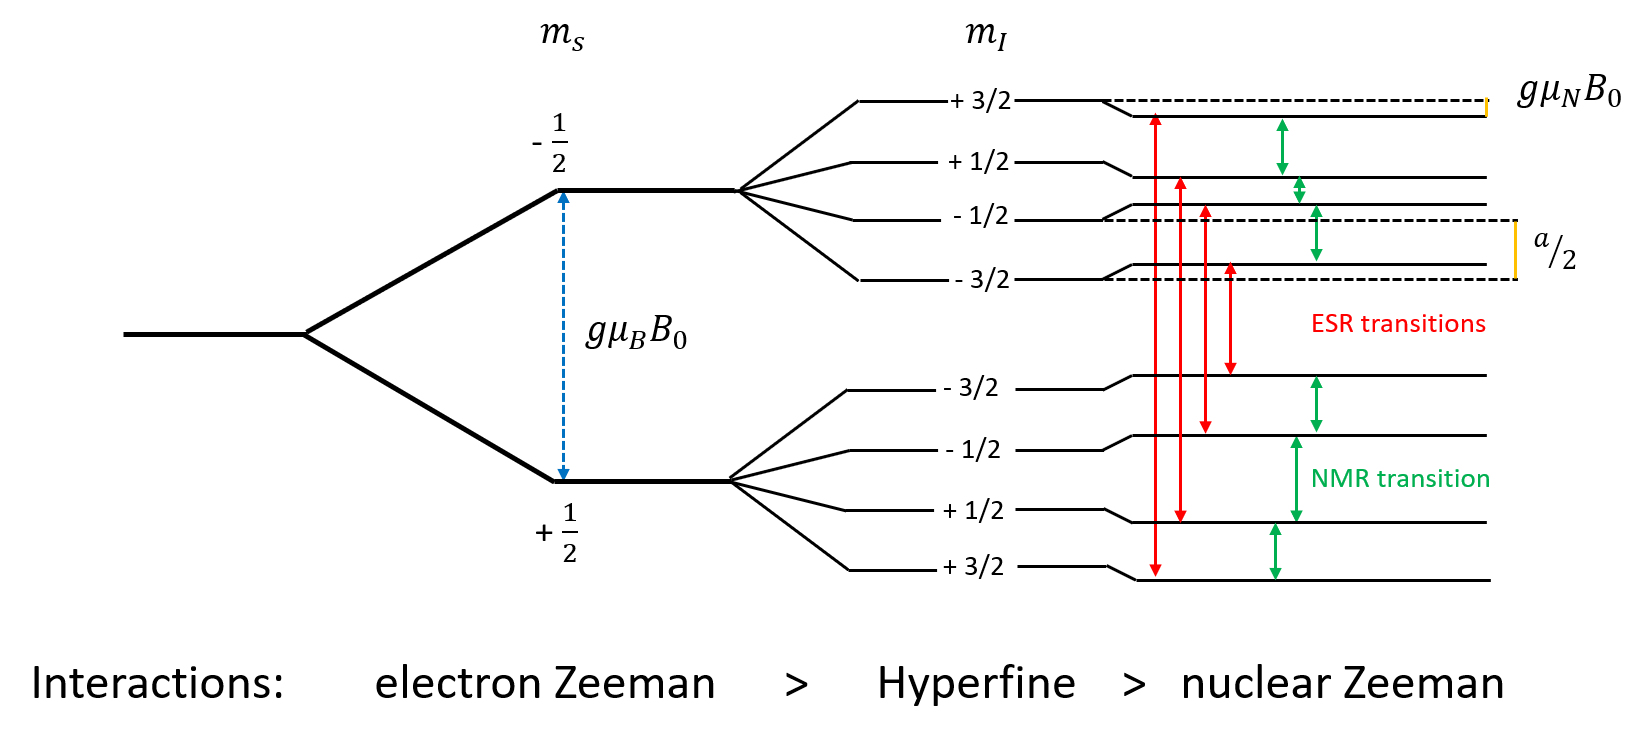
\includegraphics[height=0.32\textwidth,keepaspectratio]{hyperfinenergylevelsplitting}
\caption{\label{fig:hyperfinenergylevelsplitting} Example of an energy level diagram for a system where $S=1/2$ and $I=1/2$. The electron and nuclear Zeeman interactions terms are shown. Additionally the hyperfine interaction level splitting is shown.}
\end{figure}




%SUBSECTION HYPERFINE
\subsection{\label{sec:hyperfine}The Hyperfine Interaction}
NRI experiments can be used to probe the nuclear Zeeman splitting for spin systems where $I \neq 0$. However, there is a more significant detectable degeneracy shown in Fig.~\ref{fig:hyperfinenergylevelsplitting} which arises due to the hyperfine interaction. The hyperfine Hamiltonian term is given below as: 

\begin{equation}
\label{eq:fullzeemanhamiltonian}
\hat{H}_{HF}=\hat{\bm{S}}^{T} \bm{A} \hat{\bm{I}}
\end{equation} 

\noindent which describes the interaction between the electron and nuclear spin operators. The symmetric second-rank $\bm{A}$ tensor describes the hyperfine coupling. For an isotropic system the coupling constant is given as:

\begin{equation}
\label{eq:hyperfinestrength}
A_{o} = \frac{2\mu_{o}}{3} g\mathcal{B}_{e} g_{n}\mathcal {B}_{n}|\psi (0)|^{2} 
\end{equation} 

\noindent which gives a measure of the magnetic interaction energy between the spin particles. The electron spin density at the nucleus is given by $|\psi (0)|^{2}$.

However, if $\bm{A}$ anisotropic results in changes in the energy level splitting dependent on the orientation of the sample. The hyperfine anisotropy arises due the electron and nuclear dipole interaction. Classically this interaction energy is described by Eq.\ref{eq:classicaldipolarenergy} where $r$ is the separation distance between the unpaired electron and nucleus.


\begin{equation}
\label{eq:classicaldipolarenergy}
U_{dipolar}(\bm{r}) = \frac{\mu_{o}}{4 \pi}\left [ \frac{\bm{\mu_{e}}^{T}\cdot \bm{\mu_{n}}}{r^{3}}-\frac{3(\bm{\mu_{e}}^{T}\cdot \bm{r})(\bm{\mu_{n}}^{T}\cdot \bm{r})}{r^{5}}\right ]
\end{equation} 

\noindent $\bm{\mu_{e}}$ and $\bm{\mu_{n}}$ are the magnetic moment for the electron and nucleus, respectively. Therefore transforming to the quantum-mechanical description the Hamiltonian describing the anisotropic hyperfine interaction is:

\begin{equation}
\label{eq:quantumdipolarenergy}
\hat{H}_{dipolar}(\bm{r}) = \frac{\mu_{o}}{4 \pi} g \mathcal{B}_{n} g_{n} \mathcal{B}_{n} \left [ \frac{\hat{\bm{S}}^{T} \cdot \hat{\bm{I}}}{r^{3}}-\frac{3(\hat{\bm{S}}^{T} \cdot \bm{r} )(\hat{\bm{I}}^{T} \cdot \bm{r})}{r^{5}} \right ],
\end{equation}

\noindent which simplifies to Eq.~\ref{eq:quantumdipolarham} following integration over the electron distribution in the crystal. 

\begin{equation}
\label{eq:quantumdipolarham}
\hat{H}_{dipolar} = \hat{\bm{S}}^{T} \cdot \bm{T} \cdot \hat{\bm{I}} 
\end{equation}

\noindent Therefore the hyperfine coupling tensor is given as $\bm{A} = A_{o}\bm{\mathcal{I}_{3}} + \bm{T}$. 







%SUBSECTION PULSED EPR 
\subsection{Pulsed EPR}
\subsubsection{The Magnetisation Vector Picture}
In this section the magnetisation vector picture is used to introduce an illustration of pulse EPR experiments. In Eq.~\ref{eq:electronspinoperator} the description of the magnetic moment for a single electron is given. For a sample containing $N$ unpaired electrons with individual magnetic moments align parallel to an applied magnetic field $\textbf{B}$ whilst $\textbf{S}$ aligns anti-parallel following from Eq.~\ref{eq:electronspinoperator} gives the minimum energy. The effective macroscopic moment is $\bm{\mu}=\sum_{i}^{N} \bm{\mu_{i}}$. Therefore measurements of the spin ensemble obtains the magnetisation of the sample is given as:


\begin{equation}
\label{eq:macroscopicmagnetisation}
\textbf{M}=\frac{1}{V}\sum_{i}^{N} \bm{\mu_{i}},
\end{equation} 

\noindent which is the net magnetic moment per unit volume, $V$. An individual magnetic moment experiences a torque when in presence of a magnetic field~\citep{schweiger2001principles}:

\begin{equation}
\label{eq:torque}
\hbar \frac{d \textbf{S}}{d t}=\bm{\mu} \times \textbf{B}(t)
\end{equation} 

\noindent Therefore the ensemble magnetisation in a constant stable field $\bm{B_{0}}$ is:
\begin{equation}
\label{eq:magnetisationderiv}
\frac{d\bm{M}}{dt} = \bm{M} \times \frac{-g \mathcal{B}_{e}}{\hbar}\bm{B_{0}}.
\end{equation} 

\noindent The procession of the $\bm{M}$ around $\bm{B_{0}}$ is given by the Larmor frequency: 

\begin{equation}
\label{eq:Larmorfrequency}
\omega_{L} = \frac{g \mathcal{B}_{e} B_{0}}{\hbar},
\end{equation} 

where similarly as before $\bm{B_{0}}$ is defined as being applied along the z-axis \citep{foot2005atomic}. This description is informative as it is analogous to the precession of a spin-$\frac{1}{2}$ quantum state precessing at a rate of $\omega_{L}$ around the Bloch sphere in presence in an external magnetic field $B_{0}\bm{\hat{z}}$. 
 
\begin{figure}[h]
\centering
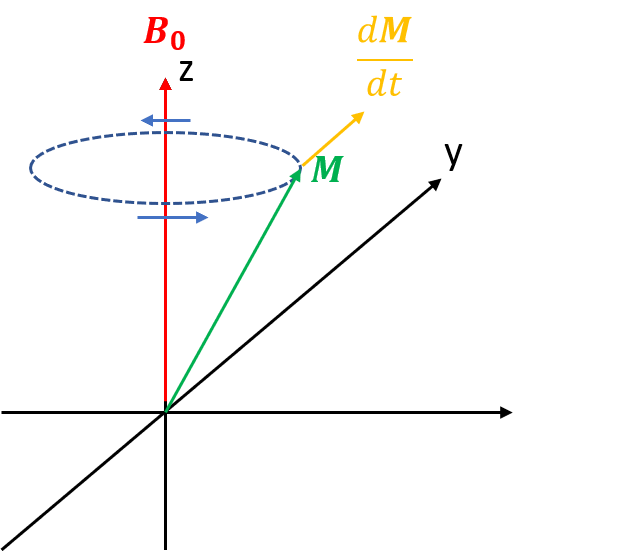
\includegraphics[height=0.32\textwidth,keepaspectratio]{magnetisationpicture}
\caption{\label{fig:magnetisationpicture} The Larmor precession of the magnetisation vector, $\bm{M}$ in the classical magnetisation vector picture.}
\end{figure}
 
 
In addition to a homogeneous magnetic field, transitions are driven between electron spin states via microwave pulses. Thus, the following provides the description of the inclusion of an oscillating magnetic field, $\bm{B_{1}}$ with a dependence on time. The components of $\bm{B_{1}}$ are:

\begin{equation}
\label{eq:magneticfieldcomponentsx}
B_{1x^{L}}(t) = B_{1}\cos(\omega_{MW}t),
\end{equation}
\begin{equation}
\label{eq:magneticfieldcomponentsy}
B_{1y^{L}}(t)=B_{1}\sin(\omega_{MW}t)
\end{equation}
\begin{equation}
\label{eq:magneticfieldcomponentsz}
B_{1z}(t) = 0.
\end{equation}
 
\noindent Following convention and describing system in the rotating frame where $\bm{B_{1}}$ is time-independent. Therefore the motion of the magnetisation in this frame is obtained by inserting $\bm{B} = \bm{B_{0}}+\bm{B_{1}}$ into Eq.~\ref{eq:magnetisationderiv}.There is an additional precession of frequency:

\begin{equation}
\label{eq:mwfieldirect}
\omega_{1}= \frac{g_{e}\mathcal{B}_{e} B_{1}}{\hbar},
\end{equation}

\noindent about the direction of $\bm{B_{1}}$.

The angle of the effective field the spins precess around is $\arctan(\omega_{1}/\Omega_{S})$ where $\Omega_{S} = \omega_{1}/\Omega_{S}$ where $\Omega_{S}= \omega_{L}-\omega_{MW}$. The spin precession rate is thus: 
\begin{equation}
\label{eq:mwfieldirecteffect}
\omega_{eff}=\sqrt{\Omega_{S}^{2}+\omega_{1}^{2}}.
\end{equation}

\noindent For the resonant case $\bm{M}$ is invariant. However, a large field effect occurs for small perturbations, where $\omega_{MW} \neq \omega_{L}$. It is now trivial to repeat the steps to calculate the effect of a linearly polarised microwave field perpendicular to $\bm{B_{0}}$, which is most likely the polarisation of the experimentally applied pulse. 




Therefore if a resonant microwave pulse is applied to the system for a time $t_{p}$ along the x-axis of the rotating frame, then magnetisation vector precessing around this axis is described as:

\begin{equation}
\label{eq:magneticfieldcomponentsx1}
M_{x}=0,
\end{equation}
\begin{equation}
\label{eq:magneticfieldcomponentsy1}
M_{y}=-M_{0}\sin(\omega_{1}t_{p}),
\end{equation}
\begin{equation}
\label{eq:magneticfieldcomponentsz1}
M_{z} = M_{0}\cos(\omega_{1}t_{p}),
\end{equation}

\noindent where for a spin system in thermal equilibrium initially $M_{0}=M_{z}$. Therefore rotation can be described by the $R_{x}(\omega_{1}t_{p})$ matrix. Therefore the rotation performed can be controlled by pulse duration, thus the combination of rotations enables rotation around a any desired axis~\citep{schweiger2001principles}.   




\subsubsection{Spin Manipulation} 
In this current picture it appears the magnetisation vector could precess for infinite amount of time around the Bloch sphere. However, this is not the case due to relaxation processes due to the interaction of a spin with it's environment. A single spin in the presence of an magnetic field will undergo longitudinal relaxation to it's thermal equilibrium state is due to stochastic processes such as phonon interactions, which is described in more detail in \label{sec:YSOdopedYbions}. In the magnetisation vector picture this relaxation mechanism is described as: 

\begin{equation}
\label{eq:mzfe}
M_{z}=M_{0}\left [ 1-2\exp{-\frac{t}{T1}} \right ],
\end{equation}

\noindent where $T_{1}$ is the decay time constant. Now considering a distribution of spin particles in the presence of $B_{0}$. Despite the aim to make $B_{0}$ completely homogeneous there will still remain a small degree of space anisotropy in the system. Therefore, the a distribution of spin will experience a slightly different $B_{0}$ field and thus will have slight different precession frequencies. This causes inhomogeneous broadening due to the frequency distribution. Spin relaxation due to inhomogeneous broadening is described by the time $T_{2}^{*}$.

The true decoherence time of the spin system is $T_{2}$ arises due to interaction of a spin with another spin which has been relaxed to the thermal equilibrium by a longitudinal relaxation mechanism. This produces the spin flip-floping process between the spins such that the upper bound of $T_{2}$:

\begin{equation}
\label{eq:T2upper}
T1 \leq 2T_{2}, 
\end{equation}

\noindent is dictated by $T_{1}$. In contrast for reversible dephasing $T_{2}^{*}$ time for the loss of quantum coherence can be refocused by applying the Hahn echo pulse sequence shown below in Fig.~\ref{fig:echopulsesequence}.

\begin{figure}[H]
    \centering
    \begin{subfigure}[b]{0.6\textwidth}
        \centering
        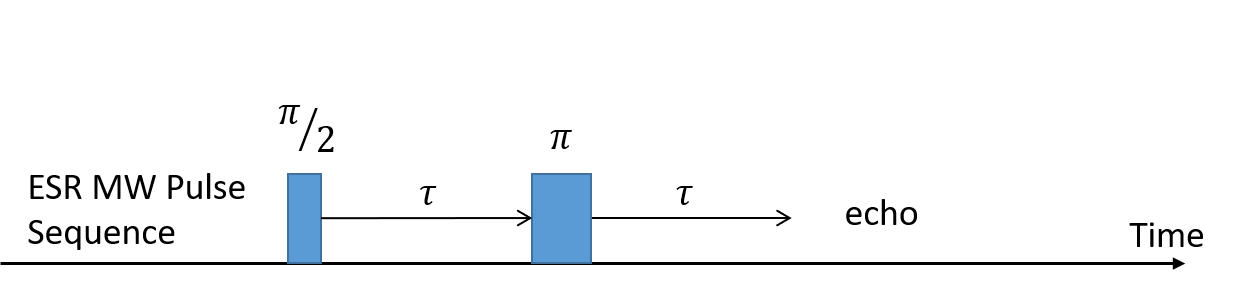
\includegraphics[width=\textwidth]{echopulsesequence}
        \caption{\label{fig:echopulsesequence}}
    \end{subfigure}
%     \hfill
    \begin{subfigure}[b]{0.6\textwidth}
        \centering
        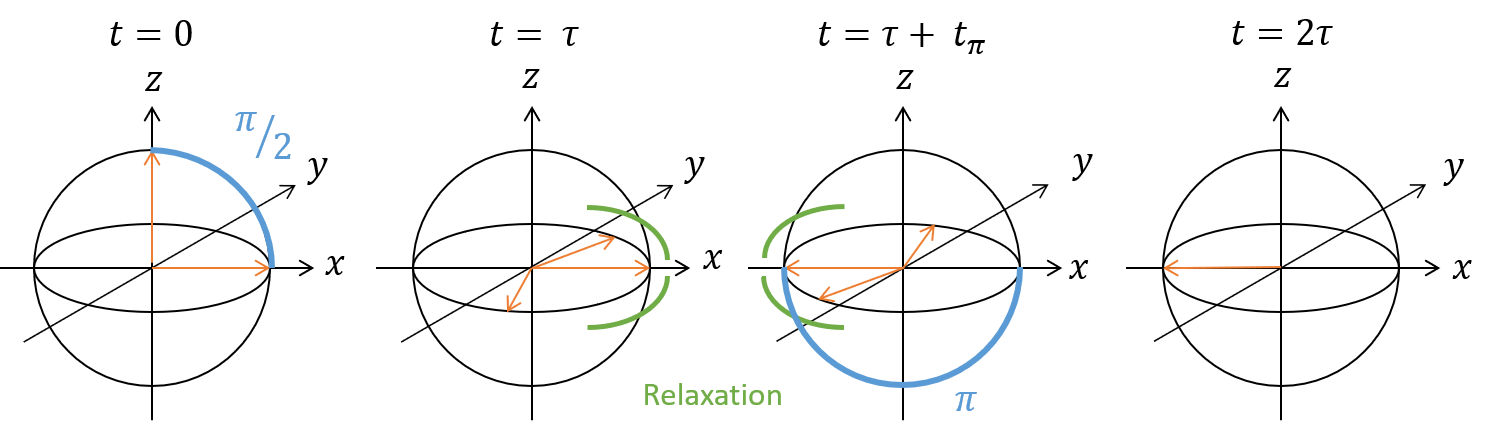
\includegraphics[width=\textwidth]{echoblochsphere}
   \caption{}
   \end{subfigure}
   \caption{(a) The Hahn echo pulse sequence. (b) Bloch sphere representation of the quantum state evolution resulting from the pulse sequence and spin dephasing.}
   \label{fig:blochsphererep}
\end{figure}

\noindent This sequence is used extensively in pulse-EPR schemes for signal detection. Additionally the inversion recovery sequence can be used to measure $T_{1}$. In this sequence shown in Fig.~\ref{fig:T1pulsesequence} an initial $\pi$-pulse is used to invert the spin state, followed by the Hahn echo pulse sequence where the time between the first $\pi$-pulse and the $\pi/2$ pulse is swept to obtain the longitudinal relaxation time. 



\begin{figure}[h]
\centering
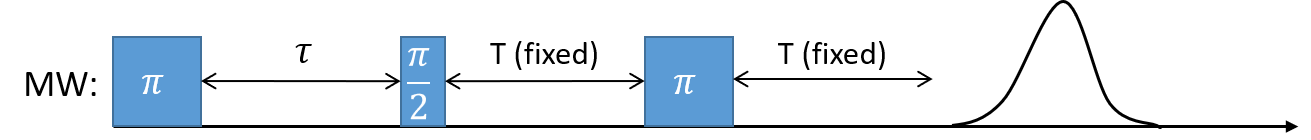
\includegraphics[height=0.05\textwidth,keepaspectratio]{T1pulsesequence}
\caption{\label{fig:T1pulsesequence} The inversion recovery pulse sequence.}
\end{figure}
 










% Recently single electron EPR held in a Penning trap. 
%v is the center frequency of the source of incident radiation

%The unitless g-factor g characterises the change in energy dependence on static magnetic
%field caused by the electron spin environment. 
%magnetic field to remove degeneracy


%schweiger:EPR gives information about the electronic structure since magnetic paramters are related to the electronic wavefunction and the configuration of surrounding nuclei with nonzero spins. 



